

\documentclass[openany,11pt,fleqn]{book} % Default font size and left-justified equations

%%%%%%%%%%%%%%%%%%%%%%%%%%%%%%%%%%%%%%%%%
% The Legrand Orange Book
% Structural Definitions File
% Version 2.0 (9/2/15)
%
% Original author:
% Mathias Legrand (legrand.mathias@gmail.com) with modifications by:
% Vel (vel@latextemplates.com)
%
% Additional modifications and partial rewrite by Brent Mellor
% 
% This file has been downloaded from:
% http://www.LaTeXTemplates.com
%
% License:
% CC BY-NC-SA 3.0 (http://creativecommons.org/licenses/by-nc-sa/3.0/)
%
%%%%%%%%%%%%%%%%%%%%%%%%%%%%%%%%%%%%%%%%%

%----------------------------------------------------------------------------------------
%	VARIOUS REQUIRED PACKAGES AND CONFIGURATIONS
%----------------------------------------------------------------------------------------

\usepackage[top=3cm,bottom=3cm,left=3cm,right=3cm,headsep=10pt,letterpaper]{geometry} % Page margins

\usepackage{graphicx} % Required for including pictures
\graphicspath{{Pictures/}} % Specifies the directory where pictures are stored

\usepackage{lipsum} % Inserts dummy text

\usepackage{tikz} % Required for drawing custom shapes

\usepackage[english]{babel} % English language/hyphenation

\usepackage{enumitem} % Customize lists
\setlist{noitemsep} % Reduce spacing between bullet points and numbered lists

\usepackage{booktabs} % Required for nicer horizontal rules in tables

\usepackage{xcolor} % Required for specifying colors by name
\definecolor{rust}{RGB}{153, 0, 0} % Define the red color used for highlighting throughout the book
\definecolor{greenrust}{RGB}{0, 153, 0} % Define the red color used for highlighting throughout the book
%----------------------------------------------------------------------------------------
%	FONTS
%----------------------------------------------------------------------------------------

\usepackage{avant} % Use the Avantgarde font for headings
%\usepackage{times} % Use the Times font for headings
\usepackage{mathptmx} % Use the Adobe Times Roman as the default text font together with math symbols from the Sym­bol, Chancery and Com­puter Modern fonts

\usepackage{microtype} % Slightly tweak font spacing for aesthetics
\usepackage[utf8]{inputenc} % Required for including letters with accents
\usepackage[T1]{fontenc} % Use 8-bit encoding that has 256 glyphs

%----------------------------------------------------------------------------------------
%	BIBLIOGRAPHY AND INDEX
%----------------------------------------------------------------------------------------

\usepackage[style=alphabetic,citestyle=numeric,sorting=nyt,sortcites=true,autopunct=true,babel=hyphen,hyperref=true,abbreviate=false,backref=true,backend=biber]{biblatex}
\addbibresource{bibliography.bib} % BibTeX bibliography file
\defbibheading{bibempty}{}

\usepackage{calc} % For simpler calculation - used for spacing the index letter headings correctly
\usepackage{makeidx} % Required to make an index
\makeindex % Tells LaTeX to create the files required for indexing



%----------------------------------------------------------------------------------------
%	MAIN TABLE OF CONTENTS
%----------------------------------------------------------------------------------------

\usepackage{titletoc} % Required for manipulating the table of contents

\contentsmargin{0cm} % Removes the default margin

% Part text styling
\titlecontents{part}[0cm]
{\addvspace{20pt}\centering\large\bfseries}
{}
{}
{}

% Chapter text styling
\titlecontents{chapter}[1.25cm] % Indentation
{\addvspace{12pt}\large\sffamily\bfseries} % Spacing and font options for chapters
{\color{rust!60}\contentslabel[\Large\thecontentslabel]{1.25cm}\color{rust}} % Chapter number
{\color{rust}}  
{\color{rust!60}\normalsize\;\titlerule*[.5pc]{.}\;\thecontentspage} % Page number

% Section text styling
\titlecontents{section}[1.25cm] % Indentation
{\addvspace{3pt}\sffamily\bfseries} % Spacing and font options for sections
{\contentslabel[\thecontentslabel]{1.25cm}} % Section number
{}
{\hfill\color{black}\thecontentspage} % Page number
[]

% Subsection text styling
\titlecontents{subsection}[1.25cm] % Indentation
{\addvspace{1pt}\sffamily\small} % Spacing and font options for subsections
{\contentslabel[\thecontentslabel]{1.25cm}} % Subsection number
{}
{\ \titlerule*[.5pc]{.}\;\thecontentspage} % Page number
[]

% List of figures
\titlecontents{figure}[0em]
{\addvspace{-5pt}\sffamily}
{\thecontentslabel\hspace*{1em}}
{}
{\ \titlerule*[.5pc]{.}\;\thecontentspage}
[]

% List of tables
\titlecontents{table}[0em]
{\addvspace{-5pt}\sffamily}
{\thecontentslabel\hspace*{1em}}
{}
{\ \titlerule*[.5pc]{.}\;\thecontentspage}
[]

%----------------------------------------------------------------------------------------
%	MINI TABLE OF CONTENTS IN PART HEADS
%----------------------------------------------------------------------------------------

% Chapter text styling
\titlecontents{lchapter}[0em] % Indenting
{\addvspace{15pt}\large\sffamily\bfseries} % Spacing and font options for chapters
{\color{rust}\contentslabel[\Large\thecontentslabel]{1.25cm}\color{rust}} % Chapter number
{}  
{\color{rust}\normalsize\sffamily\bfseries\;\titlerule*[.5pc]{.}\;\thecontentspage} % Page number

% Section text styling
\titlecontents{lsection}[0em] % Indenting
{\sffamily\small} % Spacing and font options for sections
{\contentslabel[\thecontentslabel]{1.25cm}} % Section number
{}
{}

% Subsection text styling
\titlecontents{lsubsection}[.5em] % Indentation
{\normalfont\footnotesize\sffamily} % Font settings
{}
{}
{}

%----------------------------------------------------------------------------------------
%	PAGE HEADERS
%----------------------------------------------------------------------------------------

\usepackage{fancyhdr} % Required for header and footer configuration

\pagestyle{fancy}

\renewcommand{\chaptermark}[1]{\markboth{\sffamily\normalsize\bfseries\ #1}{}} % Chapter text font settings

% \renewcommand{\sectionmark}[1]{\markright{\sffamily\normalsize\thesection\hspace{5pt}#1}{}} % Section text font settings
\fancyhf{} \fancyhead[LE,RO]{\sffamily\normalsize\thepage} % Font setting for the page number in the header
\fancyhead[LO]{\leftmark} % Print the nearest section name on the left side of odd pages
\fancyhead[RE]{\leftmark} % Print the current chapter name on the right side of even pages
\renewcommand{\headrulewidth}{0.5pt} % Width of the rule under the header
\addtolength{\headheight}{2.5pt} % Increase the spacing around the header slightly


\renewcommand{\footrulewidth}{0pt} % Removes the rule in the footer
\fancypagestyle{plain}{\fancyhead{}\renewcommand{\headrulewidth}{0pt}} % Style for when a plain pagestyle is specified

% Removes the header from odd empty pages at the end of chapters
\makeatletter
\renewcommand{\cleardoublepage}{
\clearpage\ifodd\c@page\else
\hbox{}
\vspace*{\fill}
\thispagestyle{empty}
\newpage
\fi}

%----------------------------------------------------------------------------------------
%	THEOREM STYLES
%----------------------------------------------------------------------------------------

\usepackage{amsmath,amsfonts,amssymb,amsthm} % For math equations, theorems, symbols, etc

\newcommand{\intoo}[2]{\mathopen{]}#1\,;#2\mathclose{[}}
\newcommand{\ud}{\mathop{\mathrm{{}d}}\mathopen{}}
\newcommand{\intff}[2]{\mathopen{[}#1\,;#2\mathclose{]}}
\newtheorem{notation}{Notation}[chapter]

% Boxed/framed environments
\newtheoremstyle{rustnumbox}% % Theorem style name
{0pt}% Space above
{0pt}% Space below
{\normalfont}% % Body font
{}% Indent amount
{\small\bf\sffamily\color{rust}}% % Theorem head font
{\;}% Punctuation after theorem head
{0.25em}% Space after theorem head
{\small\sffamily\color{rust}\thmname{#1}\nobreakspace\thmnumber{\@ifnotempty{#1}{}\@upn{#2}}% Theorem text (e.g. Theorem 2.1)
\thmnote{\nobreakspace\the\thm@notefont\sffamily\bfseries\color{black}---\nobreakspace#3.}} % Optional theorem note
\renewcommand{\qedsymbol}{$\blacksquare$}% Optional qed square

% Boxed/framed environments
\newtheoremstyle{rustnumbox2}% % Theorem style name
{0pt}% Space above
{0pt}% Space below
{\normalfont}% % Body font
{}% Indent amount
{\small\bf\sffamily\color{rust}}% % Theorem head font
{\;}% Punctuation after theorem head
{0.25em}% Space after theorem head
{\small\sffamily\color{greenrust}\thmname{#1}\nobreakspace\thmnumber{\@ifnotempty{#1}{}\@upn{#2}}% Theorem text (e.g. Theorem 2.1)
	\thmnote{\nobreakspace\the\thm@notefont\sffamily\bfseries\color{black}---\nobreakspace#3.}} % Optional theorem note
\renewcommand{\qedsymbol}{$\blacksquare$}% Optional qed square


\newtheoremstyle{blacknumex}% Theorem style name
{5pt}% Space above
{5pt}% Space below
{\normalfont}% Body font
{} % Indent amount
{\small\bf\sffamily}% Theorem head font
{\;}% Punctuation after theorem head
{0.25em}% Space after theorem head
{\small\sffamily{\tiny\ensuremath{\blacksquare}}\nobreakspace\thmname{#1}\nobreakspace\thmnumber{\@ifnotempty{#1}{}\@upn{#2}}% Theorem text (e.g. Theorem 2.1)
\thmnote{\nobreakspace\the\thm@notefont\sffamily\bfseries---\nobreakspace#3.}}% Optional theorem note

\newtheoremstyle{blacknumbox} % Theorem style name
{0pt}% Space above
{0pt}% Space below
{\normalfont}% Body font
{}% Indent amount
{\small\bf\sffamily}% Theorem head font
{\;}% Punctuation after theorem head
{0.25em}% Space after theorem head
{\small\sffamily\thmname{#1}\nobreakspace\thmnumber{\@ifnotempty{#1}{}\@upn{#2}}% Theorem text (e.g. Theorem 2.1)
\thmnote{\nobreakspace\the\thm@notefont\sffamily\bfseries---\nobreakspace#3.}}% Optional theorem note

% Non-boxed/non-framed environments
\newtheoremstyle{rustnum}% % Theorem style name
{5pt}% Space above
{5pt}% Space below
{\normalfont}% % Body font
{}% Indent amount
{\small\bf\sffamily\color{rust}}% % Theorem head font
{\;}% Punctuation after theorem head
{0.25em}% Space after theorem head
{\small\sffamily\color{rust}\thmname{#1}\nobreakspace\thmnumber{\@ifnotempty{#1}{}\@upn{#2}}% Theorem text (e.g. Theorem 2.1)
\thmnote{\nobreakspace\the\thm@notefont\sffamily\bfseries\color{black}---\nobreakspace#3.}} % Optional theorem note
\renewcommand{\qedsymbol}{$\blacksquare$}% Optional qed square
\makeatother

% Defines the theorem text style for each type of theorem to one of the three styles above
\newcounter{dummy} 
\numberwithin{dummy}{section}
\theoremstyle{rustnumbox}
\newtheorem{theoremeT}[dummy]{Theorem}
\newtheorem{problem}{Problem}[chapter]
\newtheorem{exerciseT}{}[chapter]
\theoremstyle{rustnumbox2}
\newtheorem{assignmentT}{}[chapter]
\theoremstyle{blacknumex}
\newtheorem{exampleT}{Example}[chapter]
\theoremstyle{blacknumbox}
\newtheorem{vocabulary}{Vocabulary}[chapter]
\newtheorem{definitionT}{Definition}[section]
\newtheorem{corollaryT}[dummy]{Corollary}
\theoremstyle{rustnum}
\newtheorem{proposition}[dummy]{Proposition}

%----------------------------------------------------------------------------------------
%	DEFINITION OF COLORED BOXES
%----------------------------------------------------------------------------------------

\RequirePackage[framemethod=default]{mdframed} % Required for creating the theorem, definition, exercise and corollary boxes

% Theorem box
\newmdenv[skipabove=7pt,
skipbelow=7pt,
backgroundcolor=black!5,
linecolor=rust,
innerleftmargin=5pt,
innerrightmargin=5pt,
innertopmargin=5pt,
leftmargin=0cm,
rightmargin=0cm,
innerbottommargin=5pt]{tBox}

% Exercise box	  
\newmdenv[skipabove=7pt,
skipbelow=7pt,
rightline=false,
leftline=true,
topline=false,
bottomline=false,
backgroundcolor=rust!10,
linecolor=rust,
innerleftmargin=5pt,
innerrightmargin=5pt,
innertopmargin=5pt,
innerbottommargin=5pt,
leftmargin=0cm,
rightmargin=0cm,
linewidth=4pt]{eBox}	

% Assignment box	  
\newmdenv[skipabove=7pt,
skipbelow=7pt,
rightline=false,
leftline=true,
topline=false,
bottomline=false,
backgroundcolor=greenrust!10,
linecolor=greenrust,
innerleftmargin=5pt,
innerrightmargin=5pt,
innertopmargin=5pt,
innerbottommargin=5pt,
leftmargin=0cm,
rightmargin=0cm,
linewidth=4pt]{aBox}	

% Definition box
\newmdenv[skipabove=7pt,
skipbelow=7pt,
rightline=false,
leftline=true,
topline=false,
bottomline=false,
linecolor=rust,
innerleftmargin=5pt,
innerrightmargin=5pt,
innertopmargin=0pt,
leftmargin=0cm,
rightmargin=0cm,
linewidth=4pt,
innerbottommargin=0pt]{dBox}	

% Corollary box
\newmdenv[skipabove=7pt,
skipbelow=7pt,
rightline=false,
leftline=true,
topline=false,
bottomline=false,
linecolor=gray,
backgroundcolor=black!5,
innerleftmargin=5pt,
innerrightmargin=5pt,
innertopmargin=5pt,
leftmargin=0cm,
rightmargin=0cm,
linewidth=4pt,
innerbottommargin=5pt]{cBox}

% Creates an environment for each type of theorem and assigns it a theorem text style from the "Theorem Styles" section above and a colored box from above
\newenvironment{theorem}{\begin{tBox}\begin{theoremeT}}{\end{theoremeT}\end{tBox}}
\newenvironment{exercise}{\begin{eBox}\begin{exerciseT}}{\hfill{\color{rust}\tiny\ensuremath{\blacksquare}}\end{exerciseT}\end{eBox}}				
\newenvironment{assignment}{\begin{aBox}\begin{assignmentT}}{\hfill{\color{greenrust}\tiny\ensuremath{\blacksquare}}\end{assignmentT}\end{aBox}}				  
\newenvironment{definition}{\begin{dBox}\begin{definitionT}}{\end{definitionT}\end{dBox}}	
\newenvironment{example}{\begin{exampleT}}{\hfill{\tiny\ensuremath{\blacksquare}}\end{exampleT}}		
\newenvironment{corollary}{\begin{cBox}\begin{corollaryT}}{\end{corollaryT}\end{cBox}}	

%----------------------------------------------------------------------------------------
%	WARNING ENVIRONMENT
%----------------------------------------------------------------------------------------

\newenvironment{warning}{\par\vspace{10pt}\small % Vertical white space above the remark and smaller font size
	\begin{list}{}{
			\leftmargin=35pt % Indentation on the left
			\rightmargin=25pt}\item\ignorespaces % Indentation on the right
		\makebox[-2.5pt]{\begin{tikzpicture}[overlay]
			\node[draw=rust!60,line width=1pt,circle,fill=rust!25,font=\sffamily\bfseries,inner sep=2pt,outer sep=0pt] at (-15pt,0pt){\textcolor{rust}{\textbf{!}}};\end{tikzpicture}} % Orange R in a circle
		\advance\baselineskip -1pt}{\end{list}\vskip5pt} % Tighter line spacing and white space after remark

%----------------------------------------------------------------------------------------
%	REMARK ENVIRONMENT
%----------------------------------------------------------------------------------------

\newenvironment{remark}{\par\vspace{10pt}\small % Vertical white space above the remark and smaller font size
\begin{list}{}{
\leftmargin=35pt % Indentation on the left
\rightmargin=25pt}\item\ignorespaces % Indentation on the right
\makebox[-2.5pt]{\begin{tikzpicture}[overlay]
\node[draw=rust!60,line width=1pt,circle,fill=rust!25,font=\sffamily\bfseries,inner sep=2pt,outer sep=0pt] at (-15pt,0pt){\textcolor{rust}{R}};\end{tikzpicture}} % Orange R in a circle
\advance\baselineskip -1pt}{\end{list}\vskip5pt} % Tighter line spacing and white space after remark

%----------------------------------------------------------------------------------------
%	SECTION NUMBERING IN THE MARGIN
%----------------------------------------------------------------------------------------

\makeatletter
\renewcommand{\@seccntformat}[1]{\llap{\textcolor{rust}{\csname the#1\endcsname}\hspace{1em}}}                    
\renewcommand{\section}{\@startsection{section}{1}{\z@}
{-4ex \@plus -1ex \@minus -.4ex}
{1ex \@plus.2ex }
{\normalfont\large\sffamily\bfseries}}
\renewcommand{\subsection}{\@startsection {subsection}{2}{\z@}
{-3ex \@plus -0.1ex \@minus -.4ex}
{0.5ex \@plus.2ex }
{\normalfont\sffamily\bfseries}}
\renewcommand{\subsubsection}{\@startsection {subsubsection}{3}{\z@}
{-2ex \@plus -0.1ex \@minus -.2ex}
{.2ex \@plus.2ex }
{\normalfont\small\sffamily\bfseries}}                        
\renewcommand\paragraph{\@startsection{paragraph}{4}{\z@}
{-2ex \@plus-.2ex \@minus .2ex}
{.1ex}
{\normalfont\small\sffamily\bfseries}}

%----------------------------------------------------------------------------------------
%	PART HEADINGS
%----------------------------------------------------------------------------------------

% numbered part in the table of contents
\newcommand{\@mypartnumtocformat}[2]{%
\setlength\fboxsep{0pt}%
\noindent\colorbox{rust!20}{\strut\parbox[c][.7cm]{\ecart}{\color{rust!70}\Large\sffamily\bfseries\centering#1}}\hskip\esp\colorbox{rust!40}{\strut\parbox[c][.7cm]{\linewidth-\ecart-\esp}{\Large\sffamily\centering#2}}}%
%%%%%%%%%%%%%%%%%%%%%%%%%%%%%%%%%%
% unnumbered part in the table of contents
\newcommand{\@myparttocformat}[1]{%
\setlength\fboxsep{0pt}%
\noindent\colorbox{rust!40}{\strut\parbox[c][.7cm]{\linewidth}{\Large\sffamily\centering#1}}}%
%%%%%%%%%%%%%%%%%%%%%%%%%%%%%%%%%%
\newlength\esp
\setlength\esp{4pt}
\newlength\ecart
\setlength\ecart{1.2cm-\esp}
\newcommand{\thepartimage}{}%
\newcommand{\partimage}[1]{\renewcommand{\thepartimage}{#1}}%
\def\@part[#1]#2{%
\ifnum \c@secnumdepth >-2\relax%
\refstepcounter{part}%
\addcontentsline{toc}{part}{\texorpdfstring{\protect\@mypartnumtocformat{\thepart}{#1}}{\partname~\thepart\ ---\ #1}}
\else%
\addcontentsline{toc}{part}{\texorpdfstring{\protect\@myparttocformat{#1}}{#1}}%
\fi%
\startcontents%
\markboth{}{}%
{\thispagestyle{empty}%
\begin{tikzpicture}[remember picture,overlay]%
\node at (current page.north west){\begin{tikzpicture}[remember picture,overlay]%	
\node[anchor=north] at (4cm,-3.25cm){\color{rust!60}\fontsize{220}{100}\sffamily\bfseries\@Roman\c@part}; 
\node[anchor=south east] at (\paperwidth-1cm,-\paperheight+1cm){\parbox[t][][t]{8.5cm}{
\printcontents{l}{0}{\setcounter{tocdepth}{1}}%
}};
\node[anchor=north east] at (\paperwidth-1.5cm,-3.25cm){\parbox[t][][t]{15cm}{\strut\raggedleft\color{black!40}\fontsize{30}{30}\sffamily\bfseries#2}};
\end{tikzpicture}};
\end{tikzpicture}}%
\@endpart}
\def\@spart#1{%
\startcontents%
\phantomsection
{\thispagestyle{empty}%
\begin{tikzpicture}[remember picture,overlay]%
\node at (current page.north west){\begin{tikzpicture}[remember picture,overlay]%	
\fill[rust!20](0cm,0cm) rectangle (\paperwidth,-\paperheight);
\node[anchor=north east] at (\paperwidth-1.5cm,-3.25cm){\parbox[t][][t]{15cm}{\strut\raggedleft\color{white}\fontsize{30}{30}\sffamily\bfseries#1}};
\end{tikzpicture}};
\end{tikzpicture}}
\addcontentsline{toc}{part}{\texorpdfstring{%
\setlength\fboxsep{0pt}%
\noindent\protect\colorbox{rust!40}{\strut\protect\parbox[c][.7cm]{\linewidth}{\Large\sffamily\protect\centering #1\quad\mbox{}}}}{#1}}%
\@endpart}
\def\@endpart{\vfil\newpage
\if@twoside
\if@openright
\null
\thispagestyle{empty}%
\newpage
\fi
\fi
\if@tempswa
\twocolumn
\fi}

%----------------------------------------------------------------------------------------
%	CHAPTER HEADINGS
%----------------------------------------------------------------------------------------

% A switch to conditionally include a picture, implemented by  Christian Hupfer
\newif\ifusechapterimage
\usechapterimagetrue
\newcommand{\thechapterimage}{}%
\newcommand{\chapterimage}[1]{\ifusechapterimage\renewcommand{\thechapterimage}{#1}\fi}%
\def\@makechapterhead#1{%
{\parindent \z@ \raggedright \normalfont
\ifnum \c@secnumdepth >\m@ne
\if@mainmatter
\begin{tikzpicture}[remember picture,overlay]
\node at (current page.north west)
{\begin{tikzpicture}[remember picture,overlay]
\node[anchor=north west,inner sep=0pt] at (0,0) {\ifusechapterimage\includegraphics[width=\paperwidth]{\thechapterimage}\fi};
%\draw[anchor=west] (\Gm@lmargin,-9cm) node [line width=2pt,rounded corners=15pt,draw=rust,fill=white,fill opacity=0.5,inner sep=15pt]{\strut\makebox[22cm]{}};

\draw[anchor=west] (\Gm@lmargin,-4cm) node [line width=2pt,rounded corners=15pt,draw=rust,fill=white,fill opacity=0.75,inner sep=15pt]{\strut\makebox[22cm]{}};

\draw[anchor=west] (\Gm@lmargin+.3cm,-4cm) node {\huge\sffamily\bfseries\color{black}\thechapter. #1\strut};
\end{tikzpicture}};
\end{tikzpicture}
\else
\begin{tikzpicture}[remember picture,overlay]
\node at (current page.north west)
{\begin{tikzpicture}[remember picture,overlay]
\node[anchor=north west,inner sep=0pt] at (0,0) {\ifusechapterimage\includegraphics[width=\paperwidth]{\thechapterimage}\fi};
%\draw[anchor=west] (\Gm@lmargin,-9cm) node [line width=2pt,rounded corners=15pt,draw=rust,fill=white,fill opacity=0.5,inner sep=15pt]{\strut\makebox[22cm]{}};

\draw[anchor=west] (\Gm@lmargin,-4cm) node [line width=2pt,rounded corners=15pt,draw=rust,fill=white,fill opacity=0.75,inner sep=15pt]{\strut\makebox[22cm]{}};

\draw[anchor=west] (\Gm@lmargin+.3cm,-4cm) node {\huge\sffamily\bfseries\color{black}#1\strut};
\end{tikzpicture}};
\end{tikzpicture}
%\fi\fi\par\vspace*{270\p@}}}

\fi\fi\par\vspace*{100\p@}}}

%-------------------------------------------

\def\@makeschapterhead#1{%
\begin{tikzpicture}[remember picture,overlay]
\node at (current page.north west)
{\begin{tikzpicture}[remember picture,overlay]
\node[anchor=north west,inner sep=0pt] at (0,0) {\ifusechapterimage\includegraphics[width=\paperwidth]{\thechapterimage}\fi};
\draw[anchor=west] (\Gm@lmargin,-9cm) node [line width=2pt,rounded corners=15pt,draw=rust,fill=white,fill opacity=0.5,inner sep=15pt]{\strut\makebox[22cm]{}};
\draw[anchor=west] (\Gm@lmargin+.3cm,-9cm) node {\huge\sffamily\bfseries\color{black}#1\strut};
\end{tikzpicture}};
\end{tikzpicture}
\par\vspace*{270\p@}}
\makeatother

%----------------------------------------------------------------------------------------
%	HYPERLINKS IN THE DOCUMENTS
%----------------------------------------------------------------------------------------

\usepackage{hyperref}
\hypersetup{hidelinks,backref=true,pagebackref=true,hyperindex=true,colorlinks=false,breaklinks=true,urlcolor= rust,bookmarks=true,bookmarksopen=false,pdftitle={Title},pdfauthor={Author}}
\usepackage{bookmark}
\bookmarksetup{
open,
numbered,
addtohook={%
\ifnum\bookmarkget{level}=0 % chapter
\bookmarksetup{bold}%
\fi
\ifnum\bookmarkget{level}=-1 % part
\bookmarksetup{color=rust,bold}%
\fi
}
}
 % Insert the commands.tex file which contains the majority of the structure behind the template
\usepackage{float}

\usepackage{listings} 
\lstset
{ 
    language=C,
    basicstyle=\ttfamily,
    columns=fullflexible,
    keepspaces=true,
    numbers=none,
    stepnumber=1,
    showstringspaces=false,
    tabsize=1,
    breaklines=true,
    breakatwhitespace=false,
    keywordstyle=\color{blue!80!black},
    stringstyle=\color{red!80!black},
    commentstyle=\color{green!40!black},
    morecomment=[l][\color{magenta!80!black}]{\#}
}

\usepackage{caption}
\captionsetup[figure]{font=small,skip=10pt}

%\usepackage{enumitem}
%\setlist{noitemsep} % or \setlist{noitemsep} to leave space around whole list


%%%%% May be too harsh to prevent paragraph breaks across pages! 
%\interlinepenalty 10000
\widowpenalties 1 10000
\raggedbottom


\newcommand{\ilcode}[1]{
    %\vspace{0.5pt}
    \smallskip
    \colorbox{gray!20!white}{
        \centering
        \parbox{\linewidth-2\fboxsep}{
            \lstinline@#1@
        }
    }
    %\vspace{0.5pt}
}

\newcommand{\code}[3]{
    \begin{figure}[]
        \colorbox{gray!20!white}{
            \parbox{\linewidth-2\fboxsep} {
                \centering 
                \lstinputlisting[language=C]{#1}
            }
        }
        \caption{#2}
        \label{#3}
    \end{figure}
}




\usepackage{textcomp}
\usepackage{wrapfig}
\usepackage{float}

\usepackage{silence} % http://ctan.org/pkg/silence
\ErrorFilter{textcomp}{Symbol \textrightarrow not provided}

% Disable paragraph indentation globally since template was indenting some and not others. (looked terrible)
%\setlength{\parindent}{0pt}


%%%%%%%%%%%%%%%%%%%%%%%%%%%%%%%%%%%%%%%%%%%%%%%%%%%%%%%%%%%%%%%%%%%%%%%%%%%%%%%%%%%%%%%%%%%%%%%%%
%%%%                                                                                         %%%%
%%%%       Chapter 2: Processor Interrupts and the NVIC Peripheral                           %%%%
%%%%                                                                                         %%%%
%%%%%%%%%%%%%%%%%%%%%%%%%%%%%%%%%%%%%%%%%%%%%%%%%%%%%%%%%%%%%%%%%%%%%%%%%%%%%%%%%%%%%%%%%%%%%%%%%

\setcounter{chapter}{1} % Manually adjust chapter counter

\begin{document}
	
\chapterimage{chapter_head_2.png} % Chapter heading image
\tableofcontents
\chapter{Hardware Interrupts and Program Flow}

\section{Overview}
This lab introduces the concept of interrupt-driven programming and guides through the configuration of interrupt-oriented peripherals; the exercises herein provide a foundation for utilizing interrupts in an embedded application. They introduce the practice of enabling, configuring parameters and writing handler routines to service peripheral interrupt requests. After completing this lab, you will understand how to use interrupts effectively without impacting the main application or each other. 

\section{\color{blue}Prelab Questions}\index{Prelab Questions}
\begin{question}[Prelab 2]
	Please answer the following questions and hand in as your prelab for Lab 2.
% The section locations for each question needs renumbering in respect to the section to which it refers
	\begin{enumerate}
		\item What is the purpose of the NVIC peripheral? %(section 3.3.1)
		\item What is the difference between interrupt tail-chaining and nesting? %(section 3.3.2) 
		\item In what file are the CMSIS libraries that control the NVIC? %(section 3.3.4)
		\item What is the purpose of the EXTI peripheral? %(section 3.4.1)
		\item What is the purpose of the SYSCFG pin multiplexers? %(section 3.4.1)
		\item What file has the defined names for interrupt numbers? %(section 3.5.1)
		\item What file has the Vector table implementation? %(section 3.2 or 3.5.2)
	\end{enumerate}
\end{question}

\section{\color{orange}Introduction to Hardware Interrupts}
% What is an interrupt
Many embedded processors\textemdash including the ARM Cortex-M0 STM32F0 family\textemdash are single-core, single-thread devices; however, many embedded applications are not a single, linear thread: these programs typically operate at low enough abstractions such that most operating system concepts\textemdash such as scheduling or multi-threading\textemdash simply do not exist. Instead, the processor hardware directly drives the program concurrency, using a method known as \textit{interrupts}. 

An interrupt is the process in which the hardware temporarily suspends the execution of the main single threaded program to execute specific regions of code at known locations in memory. We call them interrupts because these program jumps to ``interrupt'' the main program. Figure \ref{interrupt_basics} demonstrates the basic operation of an interrupt in a system such as the STM32F0. 

%(Basic interrupt operation)
\begin{figure}[h]
    \centering\includegraphics[width=\textwidth]{interrupt_basics}
    \caption{Operation of an Interrupt}
    \label{interrupt_basics}
\end{figure}

Peripherals within the embedded device typically generate these interrupts; these events signal a change in the peripheral state\textemdash such as receiving data from a communications interface. Other interrupts signal error conditions or recover from bad processor states. The user's code may use interrupts to perform operations with a higher priority than the main thread. 

Every interrupt has a hardware number designation: an interrupt's number indicates its hardware priority and indexes into the \textit{Vector Table}. The Vector Table for a processor usually exists at the beginning of the system address space and is a list of memory addresses associated with the handling of a specific interrupt. For example, the location of the RESET vector (in actuality a RESET interrupt) in the Vector Table is right at the beginning. This indicates that the first few instructions that the processor executes after power-on are a load and branch to the reset handling code. 

Whenever an interrupt triggers, the processor hardware uses the interrupt number to index into the Vector Table to find the memory address of the interrupt handling code. The processor hardware saves the current register and stack state before branching to the loaded handler address. After the routine completes, the processor restores the original state, and the main program executes almost as if no interrupt had occurred. 

Figure \ref{vector_table} (peripheral reference manual pages 217-219) shows the documentation for the STM32F072 Vector Table. The Vector Table lies within the startup assembly code for the processor; it defines human-readable names used to designate functions as the appropriate interrupt handling code. When compiling and linking, the toolchain places the address of these functions within the Vector Table data.  

\begin{figure}[]
    \centering\includegraphics[height=\textheight]{vector_table}
    \caption{STM32F072 Vector Table}
    \label{vector_table}
\end{figure}

% REVISE: how to find stuff in files will be handled later, whats in each file, remove the info here
% Talk about negative priorities and what can/cant be masked
% Talk about special-purpose interrupts

The Kiel:MDK toolchain and HAL library have already defined a few interrupt handlers within the \textit{stmstm32f0xx\_it.c} file located under the \textit{Application/User} {\textmu}Vision project folder. The device startup code and Vector Table implementation are located in the \textit{startup\_stm32f072xb.s} file within the \textit{Application/MDK-ARM} directory. These files and how to use them will be discussed throughout the lab.

% interrupt terminology
% what can generate interrupts
%   avaliable interupts in the stm32
%   location of interrupt handlers in MDK

\subsection{The SysTick Timer and Interrupt}
The SysTick timer is an important but simple peripheral within most ARM processors. It consists of a 16-bit countdown timer which starts at a software configured value; this value decrements alongside the processor clock, and reaching zero triggers an interrupt, and the peripheral resets. The SysTick interrupt is often useful as a time reference for application code, an example of this is the \texttt{HAL\_Delay()} function mentioned in the previous lab. 

Figure \ref{systick} shows how the SysTick interrupt pauses the main application to execute a small section of interrupt handler code.Due to a constant delay between successive executions of the handler, you may calculate timing accurately with longer intervals that are multiples of the SysTick period by counting the number of interrupt executions.  

\begin{figure}[h]
    \centering\includegraphics[width=\textwidth]{systick}
    \caption{Effect of the SysTick interrupt on application execution.}
    \label{systick}
\end{figure}

By default, the HAL library configures the SysTick timer to a rate of 1000 Hz, giving a 1 ms period between each interrupt. The \texttt{HAL\_Delay()} function operates by monitoring a global variable which increments within the SysTick interrupt handler; since the variable increases by one each millisecond, the delay function can stall the processor for a desired time by watching and waiting until the variable equals a calculated target amount. 


\begin{exercise}[Modifying an Existing Interrupt]
    \label{ex1}
    In this exercise, you will modify the SysTick timer interrupt to flash the blue LED on the Discovery board; you should begin this lab by generating a blank project within STMCube.
    
   \subsubsection{Preparing the Main Application}
   \begin{enumerate}
       \item Initialize all of the LED pins in the main function.
       \begin{itemize}
           \item Run-once code such as initializations should execute before the main infinite loop; never use an interrupt handler to do this!
       \end{itemize}
       \item Set the green LED (PC9) high (we will use this later in the lab)
       \item Toggle the red LED (PC6) with a moderately-slow delay (400-600ms) in the infinite loop.
       \begin{itemize}
           \item This LED indicates whether the main loop is executing; use it to determine if the system is stuck in an interrupt.
       \end{itemize} 
   \end{enumerate}
    \subsubsection{Modifying the SysTick Interrupt}
    \begin{enumerate}
        \item Find the \texttt{void SysTick\_Handler(void)} function in the \textit{stm32f0xx\_it.c} file. 
        \begin{itemize}
            \item Look under the \textit{Application/User} {\textmu}Vision project folder. 
            \item This file contains pre-generated interrupt handlers. 
        \end{itemize}
        \item Modify the SysTick handler so that it toggles the blue LED (PC7) every 200ms. 
        \begin{itemize}
            \item The HAL library uses the SysTick timer. Do not remove any pre-generated code in the handler.
        \end{itemize}
        \item The modified SysTick handler interrupts every millisecond; you can use this periodicity to count the number of iterations as a timing mechanism.
        \begin{itemize}
            \item For example, toggling an LED every 100th execution of the interrupt results in 100 ms between blinks.
            \item You will need to use either a volatile global or local-static variable to store interrupt count.
            \item \textbf{Do not use delay functions in the interrupt handler!} See warning below.
        \end{itemize}
    \item Compile and load your application onto the Discovery board. Remember to press the \textbf{RESET} button after it loads!
    \end{enumerate}

     Both the red and blue LEDs should be flashing at different rates. If the blue LED appears to stay constant and not toggle, check to ensure that you are only toggling it every 200ms.
\end{exercise}

\begin{warning}
    \textbf{\underline{Never} use any sort of delay within an interrupt handler!} Handler functions should perform work quickly and then return\textemdash the HAL delay functions will deadlock within an interrupt with the same or higher priority than the SysTick.
\end{warning}

\section{Triggering Interrupts With External Signals}
% Polling vs Interrupt/Idle Sleep

In the previous lab, we used a button press on the Discovery board to toggle between two LEDs. We did this by repeatedly checking the button state in the infinite loop of the main application; we call this method \textit{polling}. Polling has the advantage that the repetitive and periodic check enables tricks like software debouncing; it has the disadvantage, however, of using a significant number of processor cycles even when the device could otherwise sit idle. 

In some embedded systems\textemdash such as the Discovery board\textemdash wasting energy on polling is not a significant challenge as we have a constant supply of power; many battery-powered systems, however, must reduce power consumption to prolong the battery life and therefore field service.

One method of avoiding continuous polling is to leverage the interrupt system to monitor and detect changes in a pin's state; this makes it possible to place the device into a low-power mode when no other processing is necessary. 

The exercises in this lab uses the ``Wait for Interrupt'' (WFI) assembly instruction, where the processor enters into ``sleep'' mode (without changing other registers). This is the least drastic of the low-power modes that the STM32F0 offers. In this state the ARM processor stops, but all memory and peripherals operate normally. Any hardware interrupt has the capability to start the processor again; once the interrupt handler exits, the main program will continue the main application thread. 

Other low-power modes selectively shut down additional peripherals, system oscillators, and power circuitry. These modes are more limited in the methods available to wake them up\textemdash some of them may even lose device state! It is therefore imperative that you use the correct low-power mode for your application.  

\subsection{Extended Interrupts and Events Controller} \label{exti}

The \textit{Extended Interrupts and Events Controller} (EXTI) peripheral allows non-peripheral sources to trigger interrupts. While its typical use is to generate interrupts from the GPIO pins of the device, it may also monitor various internal signals such as the brownout protection circuitry (low-voltage shutdown).

The EXTI documentation begins on page 219 (Section 12.2) of the peripheral reference manual. Similar to the NVIC, bits within the EXTI registers do not feature names suggesting the signals they control. The documentation within the \textit{functional description} section on the peripheral describes the mapping between EXTI event ``lines''\textemdash input sources\textemdash and the control bits. 


\begin{itemize}
    \item \textbf{Interrupt mask register (EXTI\_IMR)}
    \begin{itemize}
        \item The IMR register ``unmasks'' or enables an input signal to generate one of the EXTI interrupts.
    \end{itemize}
    \item \textbf{Event mask register (EXTI\_EMR)}
    \begin{itemize}
        \item Processor events are similar in design to interrupts but do not cause program execution to branch to separate handler code; events generally wake the processor from low-power modes. The EMR enables input signals to generate processor events. 
    \end{itemize}
    \item \textbf{Rising trigger selection register (EXTI\_RTSR)}
    \begin{itemize}
        \item All external (pin) interrupts are edge-sensitive, which means that they only generate interrupt requests at the transitions from one logic state to another. The RTSR enables a rising/positive-edge trigger for a pin.
    \end{itemize}
    \item \textbf{Falling trigger selection register (EXTI\_FTSR)}
    \begin{itemize}
        \item The FTSR enables a negative/falling-edge trigger for a pin. The EXTI allows enabling both rising and falling triggers for inputs.  
    \end{itemize}
    \item \textbf{Software interrupt event register (EXTI\_SWIER)}
    \begin{itemize}
        \item The SWIER register allows the user to trigger any of the interrupt or event conditions within the EXTI (as long as the matching bits in the IMR or EMR registers are also set). 
    \end{itemize}
    \item \textbf{Pending register (EXTI\_PR)}
    \begin{itemize}
        \item  The pending register indicates whether an event has occurred on an input signal since the last clear. If set, the EXTI interrupt handler will trigger repeatedly until the corresponding pending flags clear. Note that some events will self-clear this bit, so manual clearing is unnecessary. 
    \end{itemize}
\end{itemize}

\begin{exercise}[Configuring the EXTI]
    \label{ex2}
   This next exercise uses the EXTI peripheral to generate interrupts on the rising-edge of the user button (PA0). Place this code in the main function \textbf{before} the infinite loop. 
    \begin{enumerate}
        \item Configure the button pin (PA0) to input-mode at low-speed, with the internal pull-down resistor enabled. 
        \item Pin PA0 connects to the EXTI input line 0 (EXTI0). 
        \begin{itemize}
            \item We will explore the relationship between pins and the EXTI input lines in the next section. 
            \item The first 16 inputs to the EXTI are for external interrupts; for example, EXTI3 is the 3rd input line.
        \end{itemize}
        \item Enable/unmask interrupt generation on EXTI input line 0 (EXTI0).
        \item Configure the EXTI input line 0 to have a rising-edge trigger.
        \begin{itemize}
            \item The peripheral reference manual documents EXTI in section 12.2 (page 219).
        \end{itemize}
    \end{enumerate}

    \noindent Due to the low-level wakeup functions it provides, the EXTI peripheral always connects to the peripheral clock, so it is not necessary to enable via the RCC.   
\end{exercise}

% What is the EXTI Peripheral 
% Main registers and operation


\subsection{Pin Multiplexing with the SYSCFG} \label{syscfg}
% SYSCFG Muxes
Although the STM32F0 family has the ability to generate external interrupts on almost any pin, only 16 available input lines connect to the EXTI; therefore, a series of pin multiplexers are necessary to select the pins that connect to the limited EXTI inputs.  

The \textit{System Configuration Controller} (SYSCFG) peripheral controls these multiplexers; the SYSCFG deals primarily with signal routing, and controls data transfer between peripherals and memory, remapping portions of memory, and some high-power communication modes. 

Figure \ref{exti_mux} shows the SYSCFG pin multiplexers that the EXTI uses; these multiplexers group external pins by their orderings within the GPIO peripherals\textemdash for example, PA0, PB0 ... PF0 are on a single multiplexer with the output routed to the EXTI0 input. 

\begin{warning}Since only a single pin from a group may be in use, select pins such that they do not conflict with each other when using multiple external interrupts. Careful planning and forethought is necessary to avoid such conflicts in your designs, but it is much simpler to address those issues before you begin programming than if you choose to address them in the later design stages.
\end{warning}

Use the EXTIx registers within the SYSCFG peripheral to configure the multiplexers. The register maps for these begin on page 177 (Section 10.1.2) of the peripheral reference manual. 

\begin{figure}[]
    \centering\includegraphics[height=0.5\textheight]{exti_mux}
    \caption{SYSCFG/EXTI Pin Multiplexers}
    \label{exti_mux}
\end{figure}

\begin{exercise}[Setting the SYSCFG Pin Multiplexer]
    \label{ex3}
    In the previous exercise you configured the EXTI to generate an interrupt on the rising edge of its input line 0. In order to get the external interrupt working with the actual button pin (PA0), you must configure the SYSCFG pin multiplexers to connect the two signals together. 
    \begin{enumerate}
        \item Use the RCC to enable the peripheral clock to the SYSCFG peripheral.
        \item Determine which SYSCFG multiplexer can route PA0 to the EXTI peripheral.
        \begin{itemize}
            \item Information about the SYSCFG is in section 10 of the peripheral reference manual (page 173).
            \item Each multiplexer indicates the input line/signal of the EXTI to which they connect.
        \end{itemize}
        \item Each of the EXTICRx registers control multiple pin multiplexers. Find which register contains the configuration bits for the required multiplexer. 
        \item Configure the multiplexer to route PA0 to the EXTI input line 0 (EXTI0).
        \begin{itemize}
            \item When accessing the EXTICRx registers in your application, you will find that they are arrays defined in \textit{stm32f0xb.h}. \\
            \ilcode{SYSCFG->EXTICR[3] |= ...   // Accesses the EXTICR4 register}
        \end{itemize} 
    \end{enumerate}
\end{exercise}


\section{Working With Interrupts}
%Figure \ref{peripherals}
Figure 1.3 in the previous lab showed a block diagram of the peripherals within an STM32F072 device. Considering that many of these peripherals can generate interrupts, the system must recognize and manage a large number of possible sources. Some peripherals share interrupts, and a single peripheral may have multiple trigger conditions.  

The large number of possible interrupt sources necessitates a way to enable, sort, and otherwise manage these sources. Because of the tight binding of the interrupts to the processor core within the ARM Cortex-M0 itself, we make use of the Nested Vectored Interrupt Controller (NVIC).

\subsection{\color{orange}The Nested Vectored Interrupt Controller}
The primary responsibilities of the NVIC are enabling and disabling interrupts, indicating requests waiting for servicing, canceling pending interrupt requests, and establishing how multiple interrupts interact through configurable priorities. Figure \ref{nvic} shows a simplified block diagram of the NVIC, also available from \textit{The Definitive Guide to Arm Cortex-M0 and Cortex-M0+ Processors}.
    
%(Graphic with NVIC taking processor-external signals and controlling the PC and register file)
\begin{figure}[h]
    \centering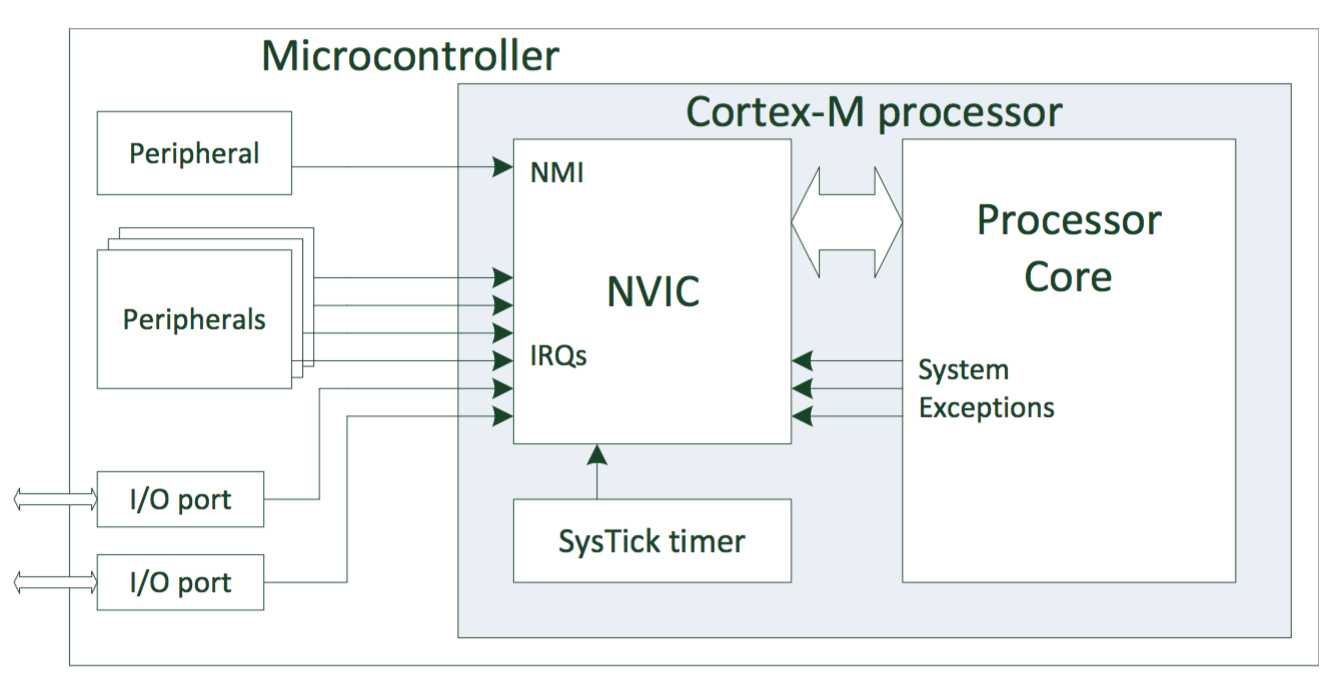
\includegraphics[width=\textwidth]{nvic}
    \caption{The Nested Vectored Interrupt Controller}
    \label{nvic}
\end{figure}

Depending on the type of ARM core within a device, the NVIC features different capabilities. Within a Cortex M0 device such as the STM32F0, the peripheral only contains the few types of control registers. Since the NVIC is a ARM-core peripheral, its documentation exists in the ARM core and programming manual\textemdash not the STM32F0 peripheral reference manual. Similarly the structure and register definitions lie within the \textit{core\_cm0.h} file, and not in the \textit{stm32f072xb.h} with the other peripherals.  

Open the core programming manual and go to page 70 (Section 4.2) which begins the register documentation for the NVIC peripheral. A summary of the NVIC registers is as follows:

\begin{itemize}
    \item \textbf{Interrupt set-enable register (ISER)}
        \begin{itemize}
            \item The ISER register enables interrupts and indicates which are active.
            Setting a bit enables the corresponding interrupt. This register is ``read and set only,'' meaning that it ignores attempts to clear bits. 
        \end{itemize}
    \item \textbf{Interrupt clear-enable register (ICER)}
        \begin{itemize}
            \item The ICER register disables interrupts.
            This register uses a write to clear scheme: setting a bit \textbf{disables} the matching interrupt. This register is ``read and write-one-clear only,'' meaning that it ignores attempts to clear bits (that is, enable interrupts). 
        \end{itemize}
    \item \textbf{Interrupt set-pending register (ISPR)}
        \begin{itemize}
            \item The ISPR shows which interrupts are pending currently; you may also set a bit in order to force a manual interrupt. 
        \end{itemize}
    \item \textbf{Interrupt clear-pending register (ICPR)}
        \begin{itemize}
            \item The ICPR shows which interrupts are pending currently, which you may manually clear; this is useful to cancel an interrupt request before the interrupt handler launches.
        \end{itemize}
    \item \textbf{Interrupt priority registers (IPR0-IPR7)}
        \begin{itemize}
            \item These registers configure the priorities for each interrupt. 
            \item Each IPR register contains four 8-bit regions to set the priority of an interrupt; the NVIC within the STM32F0 only has the uppermost two bits from these regions implemented, giving four possible configurable priority levels (0-3). More bits are available on other chipsets.           
        \end{itemize}
\end{itemize}

 
\subsection{Using CMSIS Libraries to Configure the NVIC}
Similar to ST Microelectronics, which publishes the HAL library for STM32F0 peripheral, ARM Ltd. provides the \textit{cortex microcontroller software interface standard} (CMSIS) library which controls Cortex M0 peripherals. 

Although the NVIC has a fairly simple register interface, safely modifying interrupts can become a complicated task. One of the main issues with directly modifying NVIC registers is that if an interrupt occurs during the process, it may corrupt or overwrite the register state.  

The NVIC lies within the ARM core; its interface therefore remains consistent across multiple vendors devices. This is beneficial since the CMSIS library functions usually are available regardless of the specific chip manufacturer. 

Within the exercises in these labs you have the choice of controlling the NVIC through the CMSIS library or register access. These CMSIS functions are located after the peripheral structure and register definitions in the \textit{core\_cm0.h} file. 

\subsubsection{Enabling and Setting Priorities for an Interrupt}

Using the CMSIS library functions in \textit{core\_cm0.h} simplifies configuring the NVIC. These functions identify the interrupt to be modified by a number representing its index in the Vector table. These numbers have conveniently been given defined names in the \textit{IRQn\_Type} enumeration within the \textit{stm32f072xb.h} file.  

Because the NVIC within the STM32F0 has two configuration bits for each interrupt's priority, four software priority levels are available. The CMSIS library functions accept a numeric value in the range of [0-3] as allowed priority levels. The \textbf{lower} the numerical value given, the \textbf{higher} the precedence assigned to the interrupt by the NVIC.

Think of these values as the place in line they would stand according to importance, with 0 being VIP, and 3 being a B-list celebrity (the main program code being regular people with no celebrity status).

Negative priority values for interrupts are possible, but only for specialized priority interrupts like exception and reset interrupts; this way, they \textbf{always} override user-defined interrupts.

\begin{warning}
    Remember that the highest software priority level for the NVIC is 0; the lowest is 3. The hardware priorities also follow a similar scheme with lower indexes in the Vector table having higher priority. 
\end{warning}

\begin{exercise}[Enable and Set Priority of the EXTI Interrupt]
    \label{ex4}
    Unlike most peripherals, the EXTI has multiple interrupts assigned to it. Each interrupt is bound to a selection of the EXTI input lines, and you must choose the correct to match the input line desired. 
    \begin{enumerate}
        \item In the \textit{stm32f0xb.h} file, locate the \textit{IRQn\_Type} enumeration values that reference the EXTI peripheral. 
        \begin{itemize}
            \item These are defined names for the interrupt numbers used with the CMSIS NVIC control functions.
            \item Each of the defined names for the EXTI interrupt numbers includes the range of input lines that can trigger it. 
        \end{itemize}
        \item Select the entry that references the EXTI input line 0.
        \item Enable the selected EXTI interrupt by passing its defined name to the  \texttt{NVIC\_EnableIRQ()} function. (located in \textit{core\_cm0.h})
        \item Set the priority for the interrupt to 1 (high-priority) with the \texttt{NVIC\_SetPriority()} function.
    \end{enumerate}
    
\end{exercise}

% talk about NVIC numbers in the stm32f072xb.h

% talk about avaliable priority levels
% 3- low
% 2 - medium
% 1 - high
% 0 - very high (higest)

%\begin{example}[Configuring the NVIC]
%    This example demonstrates how to enable and set the priority of an interrupt within the NVIC. 
%    
%    First we need to look up the appropriate interrupt number, preferably by a defined name in the \textit{stm32f072xb.h} file. Afterwards we can pass it to the \texttt{NVIC\_EnableIRQ()} function to enable the interrupt.
%    
%    \ilcode{NVIC\_EnableIRQ( USART1\_IRQn )}
%    
%    After enabling the interrupt, we need to set the priority. Since the USART may be receiving a stream of data, we will need some buffer unless it is possible to process each byte as it arrives. Unfortunately the USART's receive register can only hold a single byte at a time, and if new data arrives before we have read the previous byte, it will be overwritten. This means that we will have to do the buffering ourselves, and depending on the speed that the USART is configured to use, we may not have time to wait around until it becomes convenient to move the data.
%    
%    This probably means that we will want to give the USART a higher priority than many of the other interrupts. The following code snippet configures the USART interrupt to high priority.  
%    
%    \ilcode{NVIC\_SetPriority(USART1\_IRQn, 1 );  // Configure to high priority}
%    \smallskip
%\end{example}



\subsection{\color{blue}Lab Assignment: Setting up the Interrupt Handler}  \label{handler_setup}
Once you have enabled the interrupt within both the peripheral and NVIC, it is time to define a region of code as the appropriate handler. 

The MDK:ARM toolchain includes a set of function names used for interrupt handlers; the Vector table automatically reference these names when compiling and linking. Declaring a function using one of these defined names automatically makes it into an interrupt handler.

The Vector table in \textit{startup\_stm32f072xb.s} defines the names; you must declare your interrupt handlers to accept no arguments and have no return value. 

Most peripherals have a status register containing flag bits for pending interrupt requests; however, even in those without dedicated registers, most interrupts set status flags within their peripheral. These flags are necessary to generate interrupt requests. Typically you will need to clear the matching status bit manually for the interrupt condition that you are handling; otherwise, the interrupt will repeat continuously because the request never acknowledges as complete. 

\begin{warning}
    Always check the conditions for clearing status flags in the reference manual!
    
    Many status registers clear by writing a one to the bit position; others are read-only and must clear through other methods. Some peripherals such as the USART automatically clear some status flags, so clearing the flag manually is unnecessary.
\end{warning}

\begin{exercise}[Writing the EXTI Interrupt Handler]
    \label{ex5}
    This is the final step in preparing an interrupt for use. One of the biggest difficulties with using interrupts is the number of steps that you must complete correctly before getting a functioning handler.
    
    \begin{enumerate}
        \item The file \textit{startup\_stm32f072xb.s} contains the names of interrupt handlers. Find the handler name that matches the named interrupt number you found in the previous exercise. 
        \item Use the handler name to declare the handler function in either \textit{main.c} or \textit{stm32f0xx\_it.h}.
        \begin{itemize}
            \item Although pre-generated interrupt handlers exist in \textit{stm32f0xx\_it.h}, they can be anywhere within the project. 
            \item Remember that interrupt handler function declarations accept no arguments and have no return value! 
        \end{itemize}
        \item Toggle both the green and orange LEDs (PC8 \& PC9) in the EXTI interrupt handler. 
        \item Clear the appropriate flag for input line 0 in the EXTI pending register within the handler.
        \begin{itemize}
            \item Otherwise the handler will loop because the interrupt request never acknowledged.
            \item Read the bit description of the pending flags underneath the register map: these bits require a different action to clear them.
        \end{itemize}
        \item Compile and load your application onto the Discovery board.
    \end{enumerate}
    
    \noindent If you completed all the previous exercises successfully, the red and blue LEDs should continue to blink while the green and orange LEDs toggle between each other whenever the user button is pressed. 
    
    If the green and orange LEDs do not toggle, check the configuration of the EXTI and NVIC peripherals. If the red LED stops flashing and the green and orange LEDs appear to light up consistently, you are not properly clearing the pending flag in the EXTI, and your application is stuck in the EXTI interrupt handler.
    
\end{exercise}

\begin{assignment}
	Please show the TA that your green and orange LEDs toggle using an interrupt. Make sure that your passoff gets recorded on the passoff spreadsheet!
\end{assignment}

% talk about vector table defining names in startup_stm32f072xb.s

%\begin{example}[Writing the USART Interrupt Handler]
%    In the \textit{startup\_stm32f072xb.s} file, we can see the implementation of the Vector table. This table lists a series of (mostly) unimplemented function names that are linked by the toolchain whenever the appropriate interrupt request is signaled from the NVIC. 
%    
%    Looking down the table, we can find the name for the USART1 handler to be ``USART1\_IRQHandler'' We can use this name to define a function anywhere within the code project. Typically, interrupt handlers are placed either within the interrupt specific code file \textit{stm32f0xx\_it.c}, main.c, or files containing the peripheral's driver.  
%    
%    Figure \ref{usart_isr} shows a completed interrupt handler for the USART1. It begins by checking all enabled conditions to find the one triggering the interrupt, clears the condition flag, and performs some action. 
%    
%    \code{./Files/usart_isr.c}{Example USART RXNE Interrupt Handler}{usart_isr}
%    
%\end{example}

%%
%%\subsubsection{Configuring a Peripheral to Generate Interrupts} \label{periph_setup}
%%Most peripherals have multiple conditions that can trigger an interrupt. These conditions may signal different events or error states that may occur in the operation of the peripheral. Usually all interrupt-based features within a peripheral are disabled by default, this allows the user to enable only the conditions that they wish to manage in their interrupt handler. 
%%
%%\begin{example}[Enabling the USART RXNE Interrupt]
%%     In this example we'll be enabling the \textit{receive register not empty interrupt} (RXNE) which ``fires'' or triggers whenever new data arrives and is waiting to be processed. 
%%    
%%    Open the peripheral reference manual to page 720 and examine table 26.7 \textit{USART Interrupts.} This table lists all of the events that can trigger the USART interrupt. Because these events must share a single interrupt handler, they set status bits which are used to determine what event needs to be managed. The table also lists the control bits that need to be set to enable the interrupt for each specific event.
%%    
%%    From table 26.7, we can see that we need to set the \textit{RXNEIE} bit to enable the receive interrupt condition. This bit is located within the \textit{Control Register 1} (CR1) of the USART peripheral. The following line of code configures USART1 to signal an interrupt request whenever data is received
%%    
%%    \ilcode{USART1->CR1 |= USART\_CR1\_RXNEIE;   // Enable RX interrupt in USART}
%%    \smallskip
%%\end{example}


\subsection{\color{orange}Interactions Between Multiple Interrupts}
As the number of enabled interrupts within a system increases, the possibility of an interrupt request occurring during the handler of another becomes more likely; we therefore must have a deterministic way to deal with inter-interrupt interactions. The NVIC solves this problem with a system of both software configurable and fixed hardware interrupt priorities. Depending on these priority settings two outcomes are possible for multi-interrupt conditions. Figure \ref{tailChain_nesting} shows a graphical representation of each mode of operation.

\begin{figure}[]
    \centering\includegraphics[width=0.6\textwidth]{tailChain_nesting}
    \caption{Multi-Interrupt Ordering Modes}
    \label{tailChain_nesting}
\end{figure}

\subsubsection{Tail-Chaining}
Some embedded processors have only a built-in hardware ordering between interrupts. In these systems, if multiple interrupt trigger concurrently or during a handler, they execute one after each other in succession according to the hardware priority. In this mode known as \textit{tail-chaining}, interrupt handlers do not interrupt each other. Tail-chaining may use a simple save and restore mechanism for transitioning from the main thread, but it has the disadvantage of allowing a rapidly-triggering or long-running interrupt high on the hardware priority to ``starve'', or prevent lower interrupts from executing. 

The NVIC will tail-chain interrupts configured to the same software priority within the IPR registers. If multiple interrupts with the same software priority trigger simultaneously, the built-in hardware ordering determines the next handler to launch.

\subsection{\color{blue}Lab Assignment: Interrupt Nesting}
Unlike systems having only hardware interrupt priorities, the NVIC allows important interrupts to interrupt lower priority handlers; this process, called \textit{nesting}, requires a more complex context-switch mechanism but otherwise works identically to how interrupts pause execution of the main application thread. 

Allowing nested interrupts introduces some complications: some interrupt tasks require uninterrupted processing without losing or corrupting data (e.g., interrupts which move data between communication peripherals). Many of these have limited buffer space and will overwrite data if the interrupt execution delays or pauses for too long. 

Properly establishing the priorities between interrupts resolves much of the problem; in some cases, however, it may be appropriate to \textit{mask}. Masking temporarily disables other interrupts during critical sections of code. The NVIC has capabilities to mask specific interrupts, and larger relatives such as those in the Cortex M3 devices can mask interrupts by priority level. When the NVIC masks an interrupt, it may still enter the pending state; this allows the NVIC to evaluate and launch the appropriate handlers once the NVIC removes the mask.

\begin{exercise}[Long-Running Interrupts]
    \label{ex6}
   Although in some cases it may be infeasible, normally you want to keep interrupt handlers as short as possible to avoid starving parts of your program. This exercise demonstrates how a long running interrupt impacts the main application loop. 

   In this exercise we shall create a long-running interrupt by adding a delay loop to the EXTI handler you wrote earlier. \textbf{Remember, adding delay to an interrupt is typically a bad idea!} 
   \begin{enumerate}
       \item Add a delay loop of roughly 1-2 seconds to the EXTI interrupt handler.
       \begin{itemize}
           \item These exercises will temporarily break the operation of the HAL delay library.
           \item A count to 1,500,000 should be sufficient. 
       \end{itemize} 
       \item Add a second LED toggle so that the green and orange LEDs should exchange once before and after the delay loop. 
       \item Compile and load your application onto the Discovery board.
       \item Use the logic analyzer to find the time delay from the button press to the start of the interrupt routine and the LEDs changing.
       \item Take a screenshot of the result from your logic analyzer.
   \end{enumerate}
   
    \noindent When you press the user button, you should see the red LED stop flashing while the EXTI interrupt hander is in the delay loop. This indicates that the main application has stopped working since the processor is stuck in the long interrupt. 
    
   Although the main application stops whenever the system is in an interrupt handler, the SysTick handler controlling the blue LED should continue to operate normally. This is due to the priority of the SysTick handler being higher than the EXTI and therefore has the ability to interrupt the long running hander.
\end{exercise}
  
\begin{exercise}[Exploring Interrupt Priorities]
   \label{ex7}  
   In situations where you have a mix of short and long-running interrupts, pay special attention to their priorities. This exercise demonstrates how a long running interrupt can prevent others from executing properly. 
   
    \subsubsection{``Starving'' Interrupts}
    This exercise shows how having poor priority choices can prevent the SysTick handler from operating properly.  
    
    \begin{enumerate}
        \item The HAL library initializes the SysTick timer to have the highest priority possible (again, lowest numerical priority level). Add code to your main application that changes the SysTick interrupt priority to 2 (medium priority). 
        \begin{itemize}
            \item You will have to look up the defined name for the SysTick interrupt number and pass it to the \texttt{NVIC\_SetPriority()} function.
        \end{itemize} 
        \item Your EXTI interrupt should already have its priority set to 1 (high priority) in the NVIC.
        \item Compile and load your application onto the Discovery board.
    \end{enumerate}
    
    \noindent Watch the SysTick interrupt operate normally and blink the blue LED until the button is pressed and the EXTI external interrupt launches. If you set the priorities as described above, the SysTick interrupt will stop while the external interrupt operates. 
    
    What is happening in this situation? The EXTI interrupt is ``starving'' the SysTick interrupt. Determine why this is happening.

    \subsubsection{Fixing with NVIC Priorities}
    
    As shown, a long running interrupt will prevent all others of a lower or equal priority from executing until it finishes. By setting priorities properly, both interrupts can coexist. 
    
    \begin{enumerate}
        \item Change the EXTI interrupt to have priority 3. (lowest priority)
        \item Program the board and observe the LEDs, both interrupts should be working properly once more.
    \end{enumerate}
    
    In this case, it is trivial to decide on the proper priorities for the two interrupts. However, in real systems the process can become complicated. As a general rule interrupts used for timing need the highest priority, interrupts from communications peripherals need high priority, many others can be set to medium, and anything long-running should be on low. 
    
    If you must have a long-running, high-priority interrupt, verify that the others will function properly; similarly, even the lowest priority interrupts interrupt the main application thread. If your main thread performs a task, make sure you don't starve it as well.
    
\end{exercise}

\begin{assignment}
	Pass off this section with a TA to show that you are starving your interrupt; then show how changing the priorities will eliminate this problem. Note that you will need to run your program at least twice for the TA to show this change.
\end{assignment}

\section{\color{blue}Postlab Questions}\index{Postlab Questions}
\begin{question}[Postlab 2]
	Please answer the following questions and hand in as your postlab for Lab 2.
	% The section locations for each question needs renumbering in respect to the section to which it refers
	\begin{enumerate}
		\item Why can't you use both pins PA0 and PC0 for external interrupts at the same time?
		\item What software priority level gives the highest priority? What level gives the lowest?
		\item How many bits does the NVIC have reserved in its priority (IPR) registers for each interrupt (including non-implemented bits)?
		Which bits in the group are implemented?
		\item What was the latency between pushing the Discovery board button and the LED change (interrupt handler start) that you measured with the logic analyzer?
		Make sure to include a screenshot in the post-lab submission.
		\item Why do you need to clear status flag bits in peripherals when servicing their interrupts?
	\end{enumerate}
\end{question}

% Setup and enable an interrupt
%   depends on peripheral
%       enable trigger/request in peripheral
%       set priority and enable in NVIC
% Handler
%   Use default or override function stub

% Saleae Logic User Guide 
% (PDF) http://downloads.saleae.com/Saleae+Users+Guide.pdf
% (Online) http://support.saleae.com/hc/en-us/sections/201990573-saleae-users-guide
%
%\section{Lab Assignment: Writing Interrupt-Based Code}
%The following exercises explore basic concepts of interrupt-driven programming, peripheral-interrupt configuration, and how priorities order multiple interrupts. After completing these tasks, make sure to show the lab assistant! Most of your points for the lab will come from demonstrating your solutions.
%
%
%\subsubsection{Changing the Interrupt Configuration}
%Even though the HAL library has already configured the SysTick and enabled the interrupt, we are going to override the default settings in the application. 
%
%\begin{enumerate}
%    \item Use the CMSIS \texttt{SysTick\_Config()} function in your initialization code to set the SysTick interrupt rate. 
%    \begin{itemize}
%        \item The SysTick CMSIS functions are located with the NVIC control library.
%        \item The single argument to the function is the number of processor cycles the timer should count between interrupts. 
%        \begin{itemize}
%            \item This value is calculated by taking the processor clock frequency and dividing by the desired SysTick interrupt frequency. (Use 1 kHz interrupt frequency)
%            \item Since you aren't familiar with the clock system of the STM32F0, use the \texttt{HAL\_RCC\_GetHCLKFreq()} library function to get the value of the active clock source. 
%        \end{itemize}
%    \end{itemize}
%    \item Use the CMSIS functions to enable and set the priority of the SysTick interrupt in the NVIC. 
%    \begin{itemize}
%        \item See the example in section \ref{nvic_setup}.
%    \end{itemize}
%\end{enumerate}
%
%
%%\subsection{Writing an Efficient Delay Function}
%% Use SysTick to make ms delay with WFI
%
%\subsection{Using External Interrupt Sources}
%Writing a simple application based around the SysTick interrupt introduced the concepts of basic interrupt-driven programming. However, modifying the existing interrupt handler of a peripheral which requires minimal configuration doesn't give an accurate representation of the full process.  
%
%In this exercise you will be enabling an external interrupt on the rising-edge of the user button (PA0) pin. 
% 
%\begin{enumerate}
%    \item Configure the button pin (PA0) to input-mode, low-speed and with the internal pull-down resistor enabled. 
%    \item Use the RCC to enable the peripheral clock to the SYSCFG peripheral.
%    \begin{itemize}
%        \item Because of the low-level wakeup functions it can provide, the EXTI peripheral always is connected to the peripheral clock.
%    \end{itemize}
%    \item Determine and configure the SYSCFG multiplexer routing PA0 to the EXTI peripheral.
%    \begin{itemize}
%        \item See section \ref{syscfg} in the lab manual.
%        \item The SYSCFG is documented in section 10 of the peripheral reference manual. (page 173)
%        \begin{itemize}
%            \item Future labs won't provide page numbers into the documentation. You will want to get familiar with navigating the table of contents of each manual.
%        \end{itemize}
%        \item Each multiplexer indicates the input line/signal of the EXTI to which they connect.
%    \end{itemize}
%    \item Enable the external interrupt within the EXTI peripheral.
%    \begin{itemize}
%        \item See sections \ref{exti} and \ref{periph_setup} in the lab manual.
%        \item  You will need to enable/unmask the specific input line and set a rising-edge trigger.
%        \begin{itemize}
%            \item Remember that the first 16 inputs to the EXTI are used for external interrupts. For example, \textit{EXTI3} is the 3rd input line. 
%        \end{itemize}
%        \item The EXTI is documented in section 12.2 of the peripheral reference manual. (page 219, under Interrupts and Events)
%    \end{itemize}
%    \item Find the EXTI interrupt number that matches the enabled input.
%    \begin{itemize}
%        \item  See section \ref{nvic_setup} in the lab manual.
%        \item The EXTI has multiple interrupts, each of these handle a subset of its input lines.
%        \item  The defined names in the Vector table and interrupt number definitions suggest which input lines the interrupt handles.
%    \end{itemize}
%    \item Enable and configure the interrupt's priority in the NVIC.
%    \begin{itemize}
%        \item See section \ref{nvic_setup} in the lab manual.
%        \item Set the priority to be 1. (high-priority)
%    \end{itemize}
%    \item Define the interrupt handler function.
%    \begin{itemize}
%        \item See section \ref{handler_setup} in the lab manual.
%        \item Remember to clear the appropriate flag in the EXTI pending register within the handler.
%        \begin{itemize}
%            \item  Otherwise the handler will loop because the interrupt request was never acknowledged.
%        \end{itemize}
%        \item Place code that blinks or modifies the LEDs on the Discovery board within the handler.
%        \begin{itemize}
%            \item Keep in mind that the handler will trigger depending on the conditions you set in the EXTI. 
%        \end{itemize}
%    \end{itemize}
%\end{enumerate}
%
%One of the biggest difficulties with interrupts is the number of steps that need to be completed correctly before getting any positive result. 
%
%Assuming that you set a rising-edge trigger in the EXTI, you should expect to see your handler called once per button press. However, there is a good chance that you see multiple rapid transitions instead. If this occurs when pressing or releasing the button, don't worry because it's not your code.
%
%These rapid multiple triggers of the external interrupt are caused by button bounce. (see section 2.5.5 in the previous lab) The EXTI sees multiple transitions during the bouncing period and repeats the interrupt multiple times. Unfortunately, it's hard to debounce interrupts in software. Typically all interrupt lines connected to mechanical switches or buttons need hardware debouncing filters.
%
% For this lab, just ignore the bounce.
%
%% Set up EXTI interrupt
%\subsection{Measuring Interrupt Latency}
%% Use logic analyzer to measure latency of external interrupt
%In this exercise, you will be using a debugging tool known as a logic analyzer to help estimate the latency between an interrupt request and the execution of its handler. Although it isn't possible to accurately measure the individual causes, we can measure the total delay caused by the processor flushing its pipeline, loading a new address to branch, and performing operation which indicate that we've entered the interrupt handler. 
%
%If you don't you have your own Saleae logic analyzer, you can check one out from the stockroom window in the lab. You will need your U-Card as they will want to keep it until you return the device. 
%
%\subsubsection{About Logic Analyzers}
%
%The basic idea behind a logic analyzer is that it is a multi-channel digital capture tool, similar to how an oscilloscope is used to view analog signals. Unlike an oscilloscope, most logic analyzers don't capture and display data in real-time. However, even the inexpensive Saleae devices have at least four input channels and professional units may have hundreds. 
%
%Logic analyzers allow the user to capture sections of digital communications between devices. Typically you configure the device to start capturing data automatically when certain conditions are met. Afterward, the data is displayed and protocol decoders are run to annotate the data with information about what was captured.
%
%Rather than duplicate a large portion of the Saleae user manual, this lab will suggest reading portions of the online documentation throughout this exercise. The entire manual is linked here:
%\href{http://support.saleae.com/hc/en-us/sections/201990573-saleae-users-guide}{\textbf{Saleae Users Guide}}
% 
%\subsubsection{Preparing the Interrupt Handler} 
%In order to detect when the interrupt handler begins executing, we need to output some sort of physical signal that the logic analyzer can detect. The easiest method to do this is to set a pin high. When doing this we want to make sure to use an efficient method that won't waste too much time waiting for other instructions or loading and storing values from memory. 
%
%Because of this, place the provided line of code directly at the beginning of the interrupt handler before anything else. 
% 
%\ilcode{GPIOC->BSRR = 0x000003C0;   // Set all LED pins high}
%\subsubsection{Connecting and Measuring Latency}
% 
% 
% \begin{enumerate}
%     \item Familiarize yourself with the connectors on the Saleae device by reviewing the \href{http://support.saleae.com/hc/en-us/articles/210244483-Wire-Harness-Test-Clips}{\textbf{Wire Harness \& Test Clips}} section of the user guide.
%     \item Connect one of the \textit{GND} wires on the logic analyzer to a ground pin on the Discovery board.
%     \begin{itemize}
%         \item Because the Discovery board has male pin headers, you can simply push the connectors of the analyzer wires onto the pins. 
%     \end{itemize}
%     \item Connect the \textit{black} signal wire (not a black ground wire) to pin PA0 on the discovery board. This will be our indicator that the interrupt signal was requested. 
%     \item Connect the \textit{brown} signal wire to any of the LED pins on the discovery board. (PC6-PC9) . 
%     \begin{itemize}
%         \item These are our indicator that the interrupt handler has been entered.
%         \item The chosen LED needs to start cleared and should not be modified by any other interrupts. 
%     \end{itemize}
%     
%     \item Review the basics of capturing data with the \href{http://suppsort.saleae.com/hc/en-us/articles/210244503-Collecting-Data-Device-Settings}{\textbf{Collecting Data \& Device Settings}} section of the user guide.
%     \item Set a rising-edge trigger on the \textit{black} signal wire, and begin a capture session.
%     \begin{itemize}
%         \item The analyzer should open a window indicating that it is waiting for the trigger signal. 
%     \end{itemize}
%     \item Push the Discovery board button, the LEDs should appear to light instantly. 
%     \item Once the capture has finished, review the section on  \href{http://support.saleae.com/hc/en-us/articles/210244513-Measurements-Timing-Markers-and-Bookmarks}{\textbf{Measurements, Timing Markers, and Bookmarks}}.
%     \item Measure the delay between the \textit{black} signal rising-edge and the \textit{brown} signal rising-edge. 
%     \begin{itemize}
%         \item This is the estimated latency between the interrupt signal and handler execution.
%         \item Write this value down and take a screenshot of the analyzer window, you will need them for your post-lab assignment.
%     \end{itemize}
% \end{enumerate}
%
%\subsection{Exploring Interrupt Priority}
%% Change priorities of two interrupts
%Normally you want to keep interrupt handlers as short as possible. However, there are some cases where this simply isn't feasible. In situations where a long-running interrupt exists, you must pay special attention to the priorities of the others in the system. This exercise demonstrates how a long running interrupt can prevent another from executing properly. By setting appropriate priorities in the NVIC, the two interrupts can be adjusted so that they coexist without interfering with each other's operation. 
%
%To do this we are going to use both the SysTick and EXTI interrupts. Before you begin, you should have both interrupts configured and enabled in your main application.  
%
%\subsubsection{Normal Interrupt Operation}
%
%This section demonstrates how interrupts of differing priorities can operate normally with each other. 
%
%\begin{enumerate}
%    \item In each interrupt handler, write code that toggles two of the board LEDs.
%    \begin{itemize}
%        \item Make sure to use different LEDs in each handler to prevent conflicts.
%        \item Leave the priorities of the interrupt handlers the same as configured in the previous exercises.
%    \end{itemize}
%    \item Program the board and observe the LEDs.
%\end{enumerate}
%
% If both interrupts are configured correctly, the LEDs modified in the SysTick interrupt should be flashing repeatedly. If the Discovery board button is pressed, you should see the LEDs controlled by the EXTI handler update. Both interrupts should seem to be coexisting without interfering with each other. Even though they have different priorities because they run for short periods of time they don't often conflict with each other. Even if they both were to trigger at the same moment, because they are short running the impact of being delayed or paused is minor. 
%
%\subsubsection{``Starving'' Interrupts}
%Now lets change the EXTI external interrupt to simulate a long-running interrupt handler. We are going to do this by putting an infinite loop in its code. 
%
%\begin{enumerate}
%    \item Remove the previous interrupt-style LED code in the EXTI handler.
%    \item Add an infinite loop to the EXTI handler.
%    \item Write new LED code in the infinite loop as if the interrupt hander were a normal thread.
%    \begin{itemize}
%        \item The infinite loop makes the interrupt behave like an ordinary thread that never returns.
%        \item You'll need to introduce some delay into the loop to slow down the LED transitions until they are visible.
%        \item The HAL delay functions will not work within the interrupt, you must use delay loops.(section 2.5.3 in previous lab)
%        \item If you are feeling lazy you can simply turn on an LED to signal that the interrupt occurred.
%    \end{itemize}
%    \item Set the priority of the EXTI interrupt to be 1 (high priority) in the NVIC.
%    \item Set the priority of the SysTick interrupt to be 2 (medium priority) in the NVIC.
%    \item Program the board and observe the LEDs.
%\end{enumerate}
%
%After programming, watch the SysTick interrupt operate normally and blink its LEDs. Now press the button and launch the EXTI external interrupt. If you set the priorities as described above the SysTick interrupt should have frozen, while the external interrupt is operating. 
%
%What is happening in this situation? The answer is that the EXTI interrupt is ``starving'' the SysTick one. Because the EXTI interrupt runs for an extended period of time the only way the SysTick handler can occur is if it can interrupt the EXTI handler. Unfortunately, because we changed the SysTick interrupt to have a lower priority than the EXTI, it is unable to do so.
%
%Technically if the EXTI handler were to finish eventually and not continue in an infinite loop, the SysTick would eventually have the opportunity to execute, but very late.    
%
%\subsubsection{Fixing with NVIC Priorities}
%
%As shown, a long running interrupt will prevent all others of a lower or equal priority from executing until it finishes. Even though the EXTI interrupt contains an infinite loop, it is still possible to allow the SysTick to operate normally. 
%
%\begin{enumerate}
%    \item Set the priority of the SysTick interrupt to be 0 (highest priority) in the NVIC.
%    \item Program the board and observe the LEDs, both interrupts should be working properly.
%\end{enumerate}
%
%In this case, it was trivial to decide on the proper priorities for the two interrupts. However, in a real system, this process can become complicated. As a general rule interrupts used for timing need the highest priority, interrupts from communications peripherals need high priority, many others can be set to medium, and anything long-running should be on low. 
%
%If you must have a long-running, high-priority interrupt you need to be very careful to determine that the others will function properly. Likewise, even the lowest priority interrupts have higher priority than the main application thread. If your main thread performs a task, make sure it isn't getting starved as well. 
%
%Even with good priority settings, too frequent or too many interrupts can starve parts of your application. In this case, the system remains busy attempting to keep up with the flood of requests. This can cause the lowest priority portions to be perpetually pushed down on the waiting list.

\end{document}
